% !TeX program = lualatex
% Modelo de Trabalho Final de Bacharelado em Física.
% Compile da raiz do projeto com: make
\documentclass[
  12pt,
  a4paper,
  oneside,
  openany
]{abntex2}

\usepackage{babel}
\babelprovide[import,main]{brazilian}

\usepackage[T1]{fontenc}
\usepackage{lmodern}
\usepackage{microtype}
\usepackage{amsmath,amssymb,mathtools}
\usepackage{siunitx}
\usepackage{graphicx}
\usepackage{booktabs}
\usepackage{tikz}
\usepackage{pgfplots}
\pgfplotsset{compat=1.18}
\usepackage[breakable]{tcolorbox}
\usepackage{listings}
\usepackage{abntex2cite}
\usepackage{hyperref}
\usepackage{fisica}

\addto\captionsbrazilian{%
  \renewcommand{\bibname}{Referências}%
  \renewcommand{\listfigurename}{Lista de ilustrações}%
  \renewcommand{\listtablename}{Lista de tabelas}%
}

\hypersetup{
  colorlinks=false,
  pdfborder={0 0 0},
  pdftitle={Título do Trabalho Final de Bacharelado},
  pdfauthor={Nome completo do autor},
  pdfsubject={Trabalho Final de Bacharelado em Física}
}

\setlength{\parindent}{1.25cm}
\setlength{\parskip}{0pt}
\OnehalfSpacing

% Cores e ambientes compatíveis com os fragmentos reaproveitados de content/.
\definecolor{fisicabg}{HTML}{0A1020}
\definecolor{fisicacard}{HTML}{131F38}
\definecolor{fisicamuted}{HTML}{8EA3C0}
\definecolor{fisicacyan}{HTML}{5BD8E8}
\definecolor{fisicaviolet}{HTML}{B49CFF}
\definecolor{fisicaamber}{HTML}{FFC46B}
\definecolor{fisicagreen}{HTML}{7BE0A8}
\definecolor{fisicafg}{HTML}{E7EEF8}

\makeatletter
\def\frame{\@ifnextchar[{\fisica@frame@opcional}{\fisica@frame@titulo}}
\def\fisica@frame@opcional[#1]#2{\fisica@frame@titulo{#2}}
\def\fisica@frame@titulo#1{\par\subsection{#1}\begingroup\normalsize}
\def\endframe{\endgroup\par}
\makeatother
\newenvironment{columns}[1][]{\par\noindent}{\par}
\newenvironment{column}[1]{%
  \hfill\begin{minipage}[t]{#1}\vspace{0pt}
}{\end{minipage}}
\newcommand{\framesubtitle}[1]{\par\smallskip\textit{#1}\par}
\providecommand{\alert}[1]{\textbf{#1}}

\newtcolorbox{destaque}[2][fisicacyan]{%
  colback=white,
  colframe=#1,
  coltitle=black,
  title={#2},
  fonttitle=\bfseries,
  breakable
}
\newtcolorbox{equacao}{%
  colback=white,
  colframe=fisicaviolet,
  breakable
}
\lstdefinestyle{lua}{%
  language={[5.3]Lua},
  basicstyle=\ttfamily\small,
  breaklines=true,
  showstringspaces=false
}

% ---------------------------------------------------------------------
% Dados do trabalho: substitua todos os campos antes da entrega.
% ---------------------------------------------------------------------
\autor{NOME COMPLETO DO(A) AUTOR(A)}
\titulo{TÍTULO DO TRABALHO: subtítulo, se houver}
\local{CIDADE}
\data{ANO}
\orientador{Prof. Dr. Nome Completo do Orientador}
% \coorientador{Prof. Dr. Nome Completo do Coorientador}
\instituicao{%
  UNIVERSIDADE\\
  Instituto ou departamento\\
  Bacharelado em Física
}
\tipotrabalho{Trabalho de Conclusão de Curso}
\preambulo{%
  Trabalho de Conclusão de Curso apresentado ao Bacharelado em Física da
  UNIVERSIDADE, como requisito parcial para a obtenção do título de Bacharel
  em Física.
}

\begin{document}

\renewcommand{\bibname}{Referências}
\hypersetup{pageanchor=false}
\pretextual
\imprimircapa
\imprimirfolhaderosto*

% A biblioteca da instituição normalmente fornece a ficha catalográfica.
% Insira-a no verso da folha de rosto conforme as orientações locais.

\begin{folhadeaprovacao}
  \begin{center}
    \ABNTEXchapterfont\large\imprimirautor

    \vspace*{\fill}
    \begin{minipage}{0.8\textwidth}
      \begin{center}
        \ABNTEXchapterfont\bfseries\imprimirtitulo
      \end{center}
      \imprimirpreambulo
    \end{minipage}
    \vspace*{\fill}

    Aprovado em: \rule{2.5cm}{0.4pt}/\rule{2.5cm}{0.4pt}/\rule{2.5cm}{0.4pt}
  \end{center}

  \vspace*{\fill}
  \assinatura{\textbf{\imprimirorientador}\\Orientador(a)\\UNIVERSIDADE}
  \assinatura{\textbf{Nome do(a) avaliador(a) 1}\\UNIVERSIDADE}
  \assinatura{\textbf{Nome do(a) avaliador(a) 2}\\UNIVERSIDADE}
  \begin{center}
    \imprimirlocal
    \par
    \imprimirdata
  \end{center}
\end{folhadeaprovacao}

% Elementos opcionais: adapte ou remova conforme as regras do curso.
% \begin{dedicatoria}
%   \vspace*{\fill}
%   \begin{flushright}
%     Dedico este trabalho a ...
%   \end{flushright}
% \end{dedicatoria}
% \begin{agradecimentos}
%   Registre aqui os agradecimentos.
% \end{agradecimentos}
% \begin{epigrafe}
%   \vspace*{\fill}
%   \begin{flushright}
%     Texto da epígrafe.\\
%     \textit{Autoria}
%   \end{flushright}
% \end{epigrafe}

% O resumo deve ser redigido em parágrafo único; confira extensão e palavras-chave
% exigidas pelo curso. Substitua o texto de exemplo pelo resumo definitivo.
\begin{resumo}
  Este trabalho apresenta um estudo do oscilador harmônico quântico, modelo
  fundamental para a descrição de sistemas físicos próximos do equilíbrio.
  São discutidos seu espectro de energia, os estados estacionários e a
  interpretação física da energia de ponto zero. A solução é obtida pela
  equação de Schrödinger independente do tempo e comparada com a previsão
  clássica. O exemplo ilustra como hipóteses, métodos matemáticos e unidades
  físicas podem ser organizados em um trabalho de Física.

  \vspace{\onelineskip}
  \noindent\textbf{Palavras-chave}: oscilador harmônico. Mecânica quântica.
  Equação de Schrödinger.
\end{resumo}

\begin{resumo}[Abstract]
  This work presents a study of the quantum harmonic oscillator, a fundamental
  model for describing physical systems near equilibrium. Its energy spectrum,
  stationary states, and the physical interpretation of zero-point energy are
  discussed. The solution is obtained from the time-independent Schrödinger
  equation and compared with the classical prediction. This example
  illustrates how assumptions, mathematical methods, and physical units can
  be organized in a Physics thesis.

  \vspace{\onelineskip}
  \noindent\textbf{Keywords}: harmonic oscillator. Quantum mechanics.
  Schrödinger equation.
\end{resumo}

\pdfbookmark[0]{\listfigurename}{lof}
\listoffigures*
\pdfbookmark[0]{\listtablename}{lot}
\listoftables*

\begin{siglas}
  \item[ABNT] Associação Brasileira de Normas Técnicas
  \item[TFB] Trabalho Final de Bacharelado
\end{siglas}

\begin{simbolos}
  \item[$\hbar$] constante de Planck reduzida
  \item[$\hat{H}$] operador Hamiltoniano
  \item[$\psi$] função de onda
\end{simbolos}

\pdfbookmark[0]{\contentsname}{toc}
\tableofcontents*
\clearpage

\textual
\hypersetup{pageanchor=true}
\chapter{Introdução}
\label{cap:introducao}

Apresente o tema, o problema de pesquisa, a justificativa, os objetivos e a
organização do trabalho. Delimite o escopo para que as perguntas que orientam
o estudo sejam verificáveis.

\section{Motivação e aplicações}
\begin{frame}{Por que o oscilador harmônico?}
  \begin{columns}[T,onlytextwidth]
    \begin{column}{0.54\textwidth}
      \begin{itemize}
        \item Perto de um mínimo local com \alert{$V''(x_0)>0$},
              o potencial é aproximadamente parabólico:
      \end{itemize}
      \begin{equacao}
        \[
          V(x) \approx V(x_0)
          + \tfrac12 V''(x_0)\,(x-x_0)^2
        \]
      \end{equacao}
      \begin{itemize}
        \item Por isso ele descreve \alert{moléculas}, \alert{sólidos},
              \alert{campos} e \alert{circuitos}.
        \item É um dos poucos modelos quânticos com solução
              \alert{analítica exata}.
      \end{itemize}
    \end{column}
    \begin{column}{0.42\textwidth}
      \begin{destaque}{Onde ele aparece}
        \begin{itemize}
          \item Vibrações moleculares (espectroscopia IV)
          \item Fônons em cristais
          \item Íons aprisionados e qubits
          \item Ressonadores nanomecânicos
        \end{itemize}
      \end{destaque}
    \end{column}
  \end{columns}
\end{frame}

\begin{frame}{Onde isso aparece}
  \begin{columns}[T,onlytextwidth]
    \begin{column}{0.49\textwidth}
      \begin{destaque}{Moléculas diatômicas}
        Vibrações em torno do equilíbrio. As transições
        $\Delta n = \pm 1$ explicam as bandas no infravermelho.
      \end{destaque}
      \begin{destaque}[fisicaamber]{Íons aprisionados}
        O movimento de um íon em um potencial efetivo forma um
        oscilador; seus estados são usados em computação quântica.
      \end{destaque}
    \end{column}
    \begin{column}{0.49\textwidth}
      \begin{destaque}[fisicaviolet]{Circuitos supercondutores}
        Junções Josephson formam um oscilador anarmônico cujos dois
        primeiros níveis definem um qubit.
      \end{destaque}
      \begin{destaque}[fisicagreen]{Nanomecânica}
        Osciladores mecânicos levados ao estado fundamental testam
        os limites da mecânica quântica.
      \end{destaque}
    \end{column}
  \end{columns}
\end{frame}


\section{Objetivos}
\label{sec:objetivos}

O objetivo geral deste exemplo é analisar o oscilador harmônico quântico.
Como objetivos específicos, propõem-se:
\begin{itemize}
  \item formular o problema pela equação de Schrödinger;
  \item determinar e interpretar os níveis de energia;
  \item comparar as previsões quântica e clássica.
\end{itemize}

\section{Organização do trabalho}

O Capítulo~\ref{cap:fundamentacao} apresenta o referencial teórico. O
Capítulo~\ref{cap:metodologia} descreve o método, e o
Capítulo~\ref{cap:resultados} reúne os resultados e sua discussão. O
Capítulo~\ref{cap:conclusao} encerra o texto.

\chapter{Fundamentação teórica}
\label{cap:fundamentacao}

Apresentam-se os conceitos necessários para analisar o oscilador harmônico
quântico, um modelo fundamental em mecânica quântica
\cite{griffiths2018}. Extensões anarmônicas do modelo também são discutidas
na literatura \cite{bender1969}.

\section{Modelo e Hamiltoniano}

Para uma partícula de massa \(m\) sujeita a um potencial quadrático,
\begin{equation}
  V(x) = \frac{1}{2}m\omega^2x^2,
  \label{eq:potencial}
\end{equation}
em que \(\omega\) é a frequência angular. O Hamiltoniano é
\begin{equation}
  \hat{H}
  = -\frac{\hbar^2}{2m}\frac{\mathrm{d}^2}{\mathrm{d}x^2}
    + \frac{1}{2}m\omega^2x^2.
  \label{eq:hamiltoniano}
\end{equation}

\begin{frame}{Clássico versus quântico}
  \centering
  \footnotesize
  \renewcommand{\arraystretch}{1.35}
  \begin{tabular}{@{}>{\raggedright\arraybackslash}p{0.16\linewidth}
                    >{\raggedright\arraybackslash}p{0.37\linewidth}
                    >{\raggedright\arraybackslash}p{0.41\linewidth}@{}}
    \toprule
    \textbf{Aspecto} & \textbf{Clássico} & \textbf{Quântico} \\
    \midrule
    \comparacao
    \bottomrule
  \end{tabular}

  \vspace{0.7em}
  \begin{destaque}[fisicaamber]{A diferença central}
    No regime quântico a energia não pode ser zero:
    $E_0=\tfrac12\hbar\omega$.
  \end{destaque}
\end{frame}

\begin{frame}{A equação de Schrödinger}
  \begin{equacao}
    \[
      -\frac{\hbar^2}{2m}\,\frac{\mathrm{d}^2\psi}{\mathrm{d}x^2}
      + \frac12\,m\omega^2 x^2\,\psi
      = E\,\psi
    \]
  \end{equacao}

  \begin{columns}[T,onlytextwidth]
    \begin{column}{0.48\textwidth}
      \begin{destaque}{Adimensionalizar}
        \[
          \xi = \sqrt{\frac{m\omega}{\hbar}}\,x,
          \qquad
          \epsilon = \frac{2E}{\hbar\omega}
        \]
        \[
          \frac{\mathrm{d}^2\psi}{\mathrm{d}\xi^2}
          + \left(\epsilon-\xi^2\right)\psi = 0
        \]
      \end{destaque}
    \end{column}
    \begin{column}{0.48\textwidth}
      \begin{destaque}[fisicaviolet]{Condições de contorno}
        \begin{itemize}
          \item $\psi(\xi)\to 0$ quando $|\xi|\to\infty$
          \item $\psi$ e $\psi'$ contínuas
          \item Soluções normalizáveis exigem
                $\epsilon = 2n+1$
        \end{itemize}
      \end{destaque}
    \end{column}
  \end{columns}
\end{frame}

\begin{frame}{Espectro de energia}
  \begin{equacao}
    \[
      E_n = \left(n+\frac12\right)\hbar\omega,
      \qquad n = 0,1,2,\ldots
    \]
  \end{equacao}

  \begin{columns}[T,onlytextwidth]
    \begin{column}{0.53\textwidth}
      \begin{itemize}
        \item Níveis \alert{igualmente espaçados}:
              $\Delta E = \hbar\omega$.
        \item O estado fundamental tem energia \alert{não nula}.
      \end{itemize}
      \begin{destaque}{Energia de ponto zero (via Lua)}
        Para $\hbar\omega = 250\ \mathrm{meV}$:
        \[
          E_0 = \frac12\hbar\omega = \energia{0}{250}
        \]
      \end{destaque}
    \end{column}
    \begin{column}{0.44\textwidth}
      \begin{destaque}[fisicaamber]{Consequência}
        Mesmo a $T=0$ o oscilador não está em repouso. Essa energia
        residual é exigida pelo princípio da incerteza e tem efeitos
        mensuráveis em vibrações moleculares e em qubits.
      \end{destaque}
    \end{column}
  \end{columns}
\end{frame}


\chapter{Metodologia}
\label{cap:metodologia}

Descreva como o problema foi investigado para permitir que outra pessoa
reproduza o procedimento. Informe as hipóteses, condições iniciais ou de
contorno, parâmetros, instrumentos, algoritmos e critérios de análise
pertinentes ao trabalho.

\section{Procedimento de solução}

Neste exemplo, resolve-se a equação de Schrödinger independente do tempo
para o potencial harmônico \(V(x)\). Identifique as aproximações empregadas
e justifique por que são adequadas aos objetivos.

\begin{frame}{Constantes físicas via Lua}
  \centering
  \footnotesize
  \renewcommand{\arraystretch}{1.2}
  \begin{tabular}{@{}lll@{}}
    \toprule
    \textbf{Símbolo} & \textbf{Valor (CODATA 2022)} & \textbf{Grandeza} \\
    \midrule
    \tabelaconstantes{c,hbar,e,me,mp,kB}
    \bottomrule
  \end{tabular}

  \vspace{0.8em}
  \begin{destaque}{Como funciona}
    \small
    \texttt{\textbackslash tabelaconstantes\{...\}} lê
    \texttt{lua/constantes.lua} e imprime linhas formatadas pelo
    \texttt{siunitx}. Alterar um valor no Lua atualiza o TFB e os slides.
  \end{destaque}
\end{frame}

\begin{frame}[fragile]{Como o template usa Lua}
  \begin{columns}[T,onlytextwidth]
    \begin{column}{0.45\textwidth}
      \begin{destaque}{Um módulo, três usos}
        \begin{itemize}
          \item Constantes e unidades
          \item Tabelas e listas de exercícios
          \item CSV $\rightarrow$ gráficos \texttt{pgfplots}
        \end{itemize}
      \end{destaque}
      \begin{destaque}[fisicaviolet]{Compilar}
        \small
        \texttt{make} compila o TFB\\[2pt]
        \texttt{make slides} compila a apresentação
      \end{destaque}
      {\scriptsize\color{fisicamuted}%
       No texto: \texttt{\textbackslash cte\{hbar\}} e
       \texttt{\textbackslash energia\{0\}\{250\}}.}
    \end{column}
    \begin{column}{0.52\textwidth}
      \begin{lstlisting}[style=lua]
-- lua/fisica.lua (trecho)
function M.constante(chave)
  local c = constantes.obter(chave)
  tex.sprint(string.format(
    "$%s = \\qty{%s}{%s}$",
    c.simbolo,
    c.valor,
    c.unidade))
end
      \end{lstlisting}
    \end{column}
  \end{columns}
\end{frame}


\chapter{Resultados e discussão}
\label{cap:resultados}

Apresente os resultados de forma organizada e discuta sua relação com os
objetivos e com a literatura. Não substitua a análise por uma sequência de
figuras ou tabelas: explique o que cada resultado mostra e quais são suas
limitações.

\section{Espectro de energia}

Para o oscilador harmônico quântico, os níveis de energia são
\begin{equation}
  E_n = \hbar\omega\left(n+\frac{1}{2}\right),
  \qquad n=0,1,2,\ldots.
  \label{eq:energia}
\end{equation}
Em particular, o estado fundamental possui energia não nula,
\(E_0=\hbar\omega/2\).

\begin{table}[htbp]
  \centering
  \caption{Primeiros níveis de energia do oscilador harmônico}
  \label{tab:niveis}
  \begin{tabular}{cccc}
    \toprule
    \(n\) & \(E_n\) & Paridade & Nós \\
    \midrule
    \niveisTabela
    \bottomrule
  \end{tabular}
  \fonte{Elaboração própria; dados calculados em \texttt{lua/conteudo.lua}
  para \(\hbar\omega=\qty{250}{\milli\electronvolt}\).}
\end{table}

\begin{frame}{Funções de onda}
  \framesubtitle{Soluções normalizadas sobre o potencial parabólico}
  \begin{columns}[T,onlytextwidth]
    \begin{column}{0.35\textwidth}
      \begin{destaque}{Forma geral}
        \[
          \psi_n(\xi) = N_n\,H_n(\xi)\,e^{-\xi^2/2}
        \]
        {\scriptsize\color{fisicamuted}%
         $N_n=(2^n n!\sqrt{\pi})^{-1/2}$,\quad
         $\xi=\sqrt{m\omega/\hbar}\,x$}
      \end{destaque}
      \begin{itemize}
        \item $n$ nós e paridade $(-1)^n$
        \item $|\psi_n|^2$: densidade de probabilidade
      \end{itemize}
    \end{column}
    \begin{column}{0.62\textwidth}
      \centering
      \begin{tikzpicture}
        \begin{axis}[
          width=\linewidth,
          height=5.55cm,
          axis lines=left,
          axis line style={draw=fisicamuted,line width=0.5pt},
          xmin=-4.1, xmax=4.1,
          ymin=0, ymax=5.7,
          xlabel={$x\,/\,\sqrt{\hbar/m\omega}$},
          ylabel={$E\,/\,\hbar\omega$},
          xlabel style={font=\scriptsize,text=fisicamuted},
          ylabel style={font=\scriptsize,text=fisicamuted},
          tick label style={font=\scriptsize,text=fisicamuted},
          grid=major,
          grid style={draw=fisicamuted!12},
          legend style={
            at={(0.03,0.97)},anchor=north west,
            draw=none,fill=fisicabg,fill opacity=0.85,text opacity=1,
            text=fisicafg,font=\scriptsize,row sep=0pt},
          legend cell align=left,
        ]
          \plotOscilador
        \end{axis}
      \end{tikzpicture}
    \end{column}
  \end{columns}
\end{frame}


\begin{figure}[htbp]
  \centering
  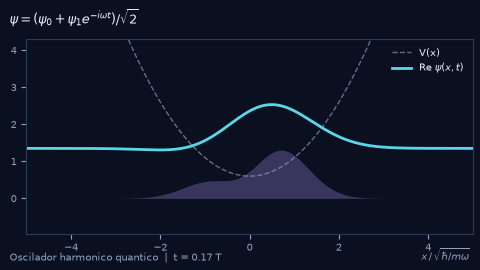
\includegraphics[width=0.8\textwidth]{videos/demo-oscilador.png}
  \caption{Visualização de uma superposição de estados do oscilador
  harmônico quântico}
  \label{fig:exemplo}
  \fonte{Material de demonstração incluído no repositório.}
\end{figure}

\chapter{Conclusão}
\label{cap:conclusao}

Retome os objetivos e responda ao problema de pesquisa com base nos
resultados apresentados. Sintetize as contribuições, explicite limitações
e, se pertinente, indique possibilidades de continuidade. Não introduza
resultados inéditos nesta seção.

\section{Síntese}
\begin{frame}{Resumo}
  \begin{columns}[T,onlytextwidth]
    \begin{column}{0.49\textwidth}
      \begin{destaque}{O que vimos}
        \begin{itemize}
          \item Potencial parabólico $\Rightarrow$ modelo exato
          \item $E_n=\left(n+\tfrac12\right)\hbar\omega$
          \item Funções de onda com paridade definida
        \end{itemize}
      \end{destaque}
    \end{column}
    \begin{column}{0.49\textwidth}
      \begin{destaque}[fisicagreen]{Próximos passos}
        \begin{itemize}
          \item Operadores de criação e destruição
          \item Oscilador em $3$D e degenerescência
          \item Oscilador forçado e dissipação
        \end{itemize}
      \end{destaque}
    \end{column}
  \end{columns}

  \vspace{0.5em}
  \begin{equacao}
    \[
      \hat a = \sqrt{\frac{m\omega}{2\hbar}}
      \left(\hat x + \frac{\iu}{m\omega}\,\hat p\right),
      \qquad
      \comm{\hat a}{\hat a^\dagger} = 1
    \]
  \end{equacao}
\end{frame}



\postextual
\bibliographystyle{abntex2-num}
\bibliography{referencias}

\begin{apendicesenv}
\partapendices
\chapter{Derivação complementar}
\label{ap:derivacao}

Use apêndices para materiais produzidos pelo autor que complementem o texto,
como demonstrações extensas, código ou questionários. Se não houver conteúdo
que justifique um apêndice, remova este arquivo e o ambiente correspondente
de \texttt{main.tex}.

Como exemplo, a substituição
\[
  \xi = \sqrt{\frac{m\omega}{\hbar}}\,x
\]
na equação de Schrödinger permite expressá-la em uma variável adimensional.
Apresente aqui os passos algébricos completos quando eles forem úteis à
reprodução do resultado, mas excessivamente longos para o capítulo principal.

\section{Exercícios propostos}
\begin{frame}{Exercícios}
  \small
  \setlength{\itemsep}{0.55em}
  \begin{enumerate}
    \exercicios
  \end{enumerate}

  \vfill
  {\scriptsize\color{fisicamuted}%
   Lista montada a partir de \texttt{lua/conteudo.lua}.}
\end{frame}


\end{apendicesenv}

% Anexos são documentos não elaborados pelo autor. Descomente e crie o arquivo
% correspondente somente se o trabalho realmente tiver anexos.
% \begin{anexosenv}
% \partanexos
% \include{capitulos/anexo-exemplo}
% \end{anexosenv}

\end{document}
